\documentclass[a4paper]{article}
\usepackage[top=1cm,bottom=2cm,left=2cm,right=2cm]{geometry}
\usepackage{multicol,caption}
\usepackage{lipsum}
\usepackage{graphicx}
\usepackage[parfill]{parskip}
\usepackage{authblk}
\usepackage{titlesec}
\usepackage{wrapfig}
\usepackage[utf8]{inputenc}
\usepackage{lipsum}
\usepackage{tikz}
\usepackage{chemfig}

\renewcommand{\figurename}{Abbildung}

\newbox\one
\newbox\two
\long\def\loremlines#1#2{
	\setbox\one=\vbox {
		\lipsum[#1]
	}
	\setbox\two=\vsplit\one to #2\baselineskip
	\unvbox\two}

\newenvironment{Figure}
	{\par\medskip\noindent\minipage{\linewidth}}
	{\endminipage\par\medskip}

\titlespacing*{\section}
{0pt}{1.0ex plus 1ex minus .2ex}{0.0ex plus .2ex}
\titlespacing*{\subsection}
{0pt}{1.0ex plus 1ex minus .2ex}{0.0ex plus .2ex}
\titlespacing*{\subsubsection}
{0pt}{0.5ex plus 1ex minus .2ex}{0.0ex plus .2ex}

\title{NMR Spektroskopie Praktikumsbericht}
\author{Andreas Bachmann, André de Jesus Morgado, Simon de Montmollin
	\\
	ZHAW Zurich University of Applied Sciences\\
	School of Engineering
}
\date{10.05.2018}


\begin{document}
	\maketitle
	
	%Body
	\begin{multicols*}{2}
		\section{Einleitung}
			\loremlines{5}{4}
			
			\begin{Figure}
				\centering
				\begin{tikzpicture}
				\node[anchor=south west,inner sep=0] at (1cm,0.5cm) {
					\chemfig{C([:270]-C*6(=C(-H)-C(-H)=C(-H)-C(-H)=C(-H)-))(-[:200]H)(-[:160]H)([:45]-C([:135]-H)([:45]-H)([:315]-H))}
				};
				\node (A1) at (0.5cm,0.5cm) {\huge I};
				\node (A2) at (3cm,0cm) {\large Aromatischer Ring};
				\node (B1) at (0cm,6.25cm) {\huge II};
				\node (B2) at (0.5cm,5cm) {\large \chemfig{CH_2}};
				\node (C1) at (6cm,6.5cm) {\huge III};
				\node (C2) at (5.75cm,5.25cm) {\large \chemfig{CH_3}};
				\end{tikzpicture}
				\captionof{figure}{XXX}
				\label{fig:xray}
				\vspace*{4mm}
			\end{Figure}
		
			\loremlines{6}{4}
		
		\section{MAS-Rotor Testen}
			\subsection{Methode}
				\loremlines{10}{4}
				
				\begin{Figure}
					\centering
					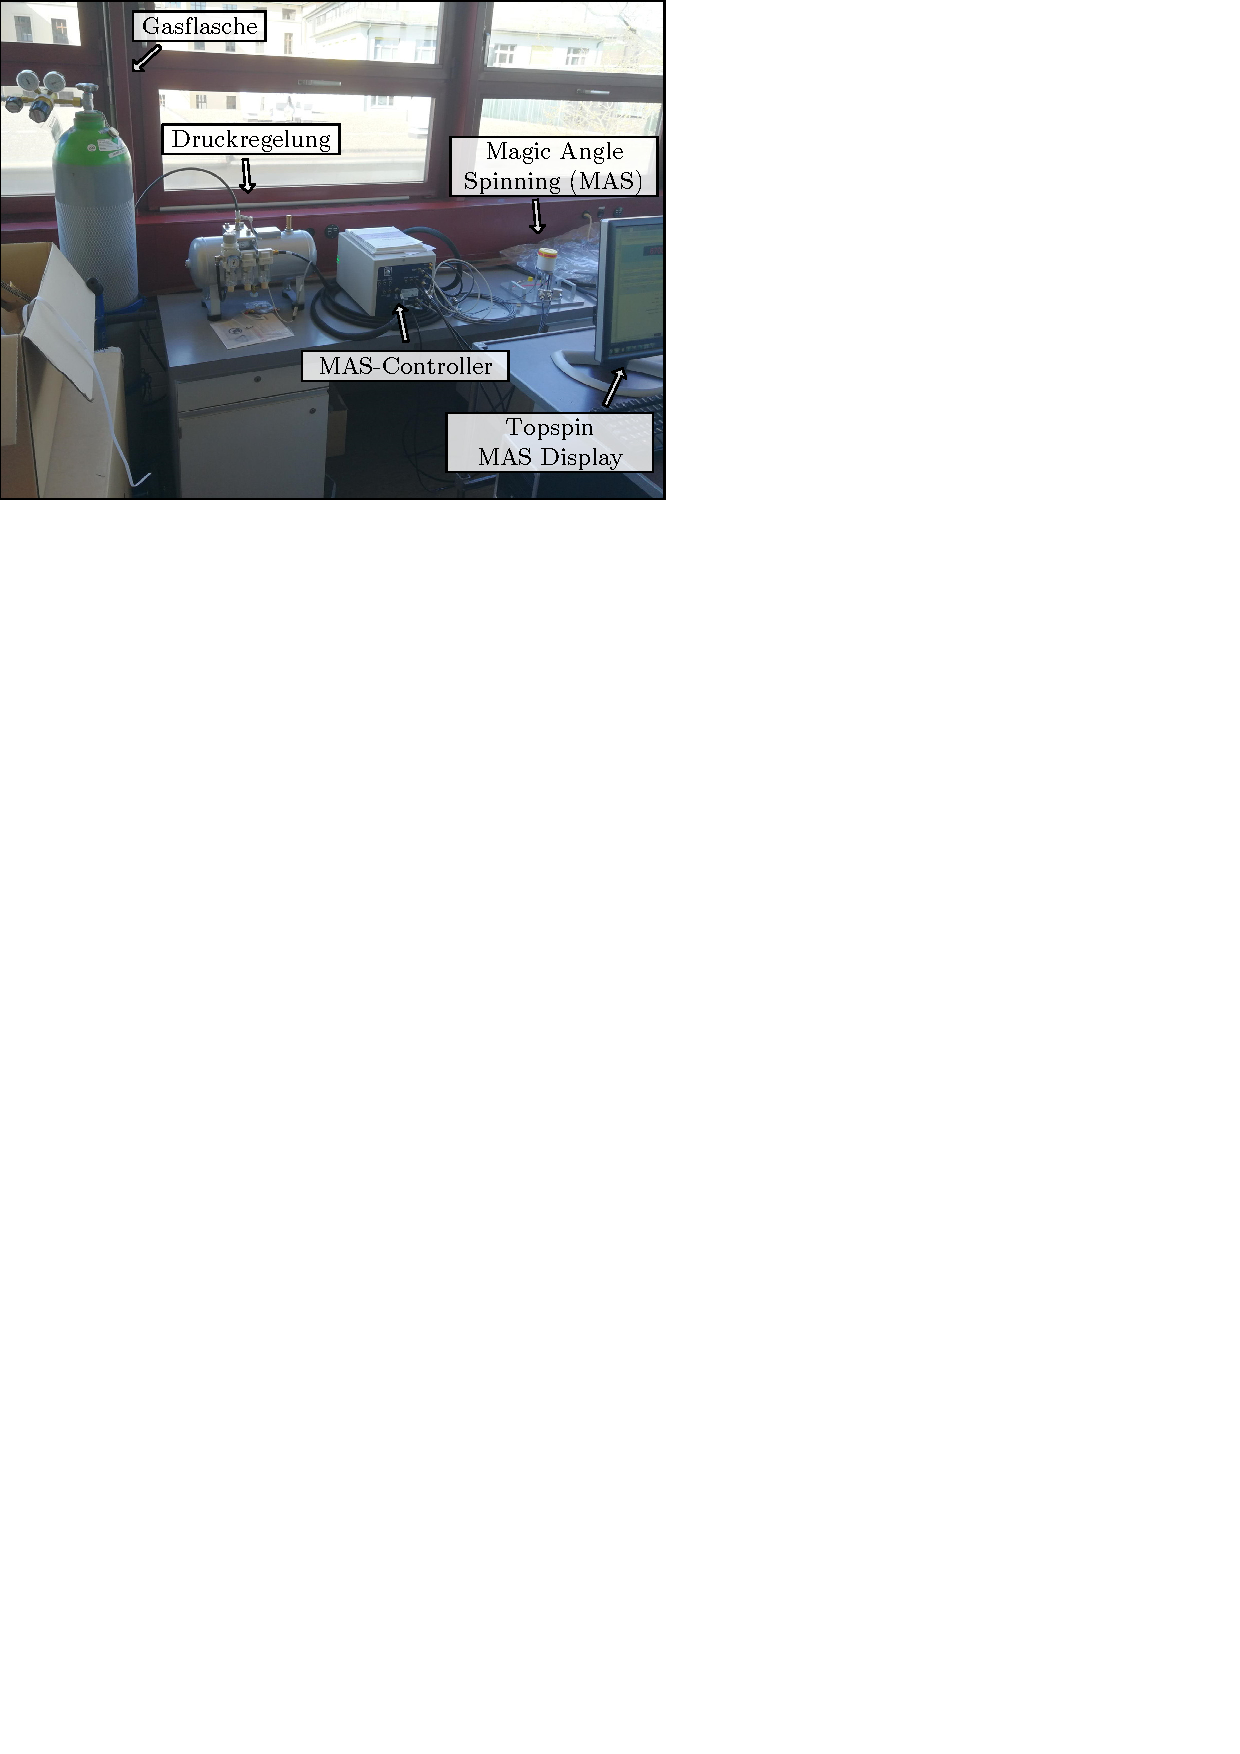
\includegraphics[trim={0cm 21.2cm 9.7cm 0},clip,width=8cm]{images/Device_2.pdf}
					\captionof{figure}{YYY}
					\label{fig:xray}
					\vspace*{4mm}
				\end{Figure}
				
				\loremlines{13}{4}
				
				\begin{Figure}
					\centering
					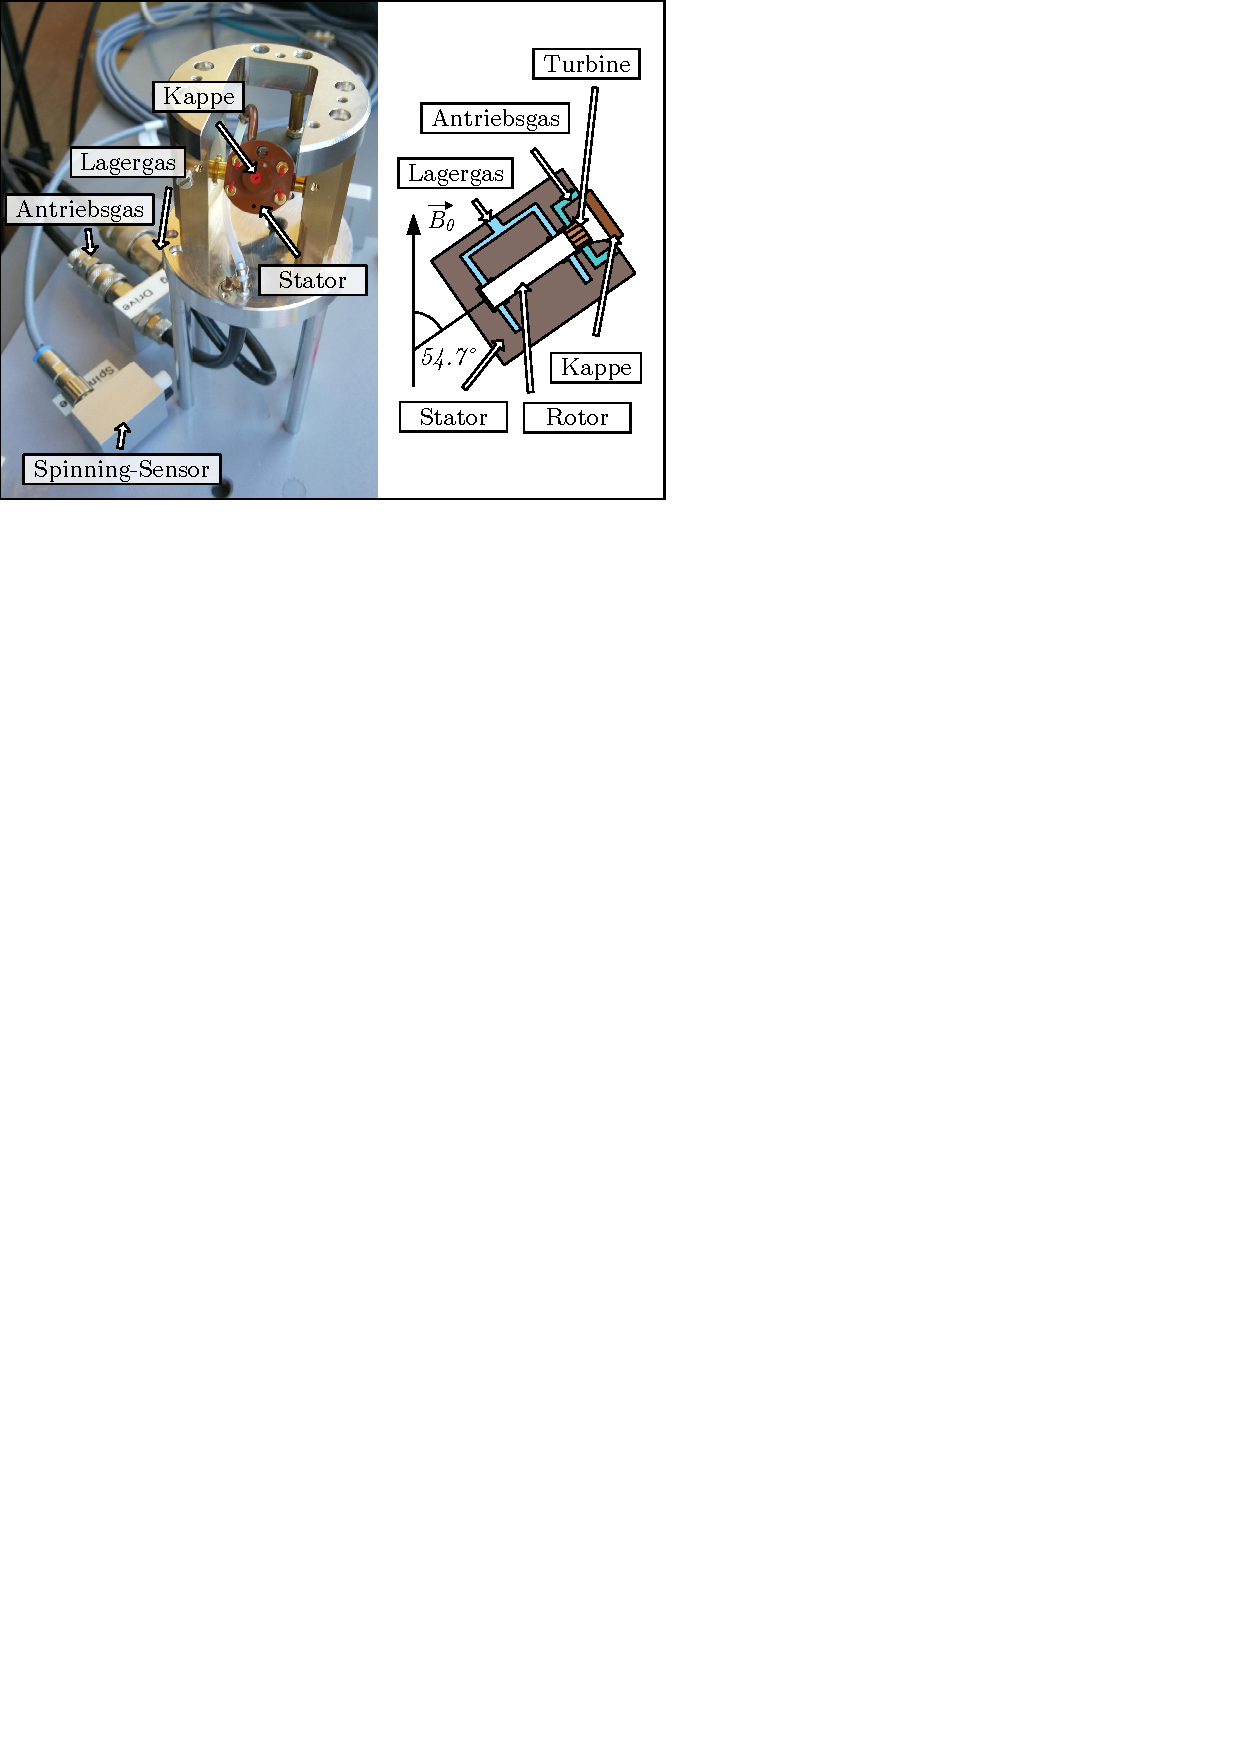
\includegraphics[trim={0cm 21.2cm 9.7cm 0},clip,width=8cm]{images/Device_3.pdf}
					\captionof{figure}{ZZZ}
					\label{fig:xray}
					\vspace*{4mm}
				\end{Figure}
				
			\subsection{Resultate}
				\loremlines{11}{8}
				
				\begin{Figure}
					\centering
					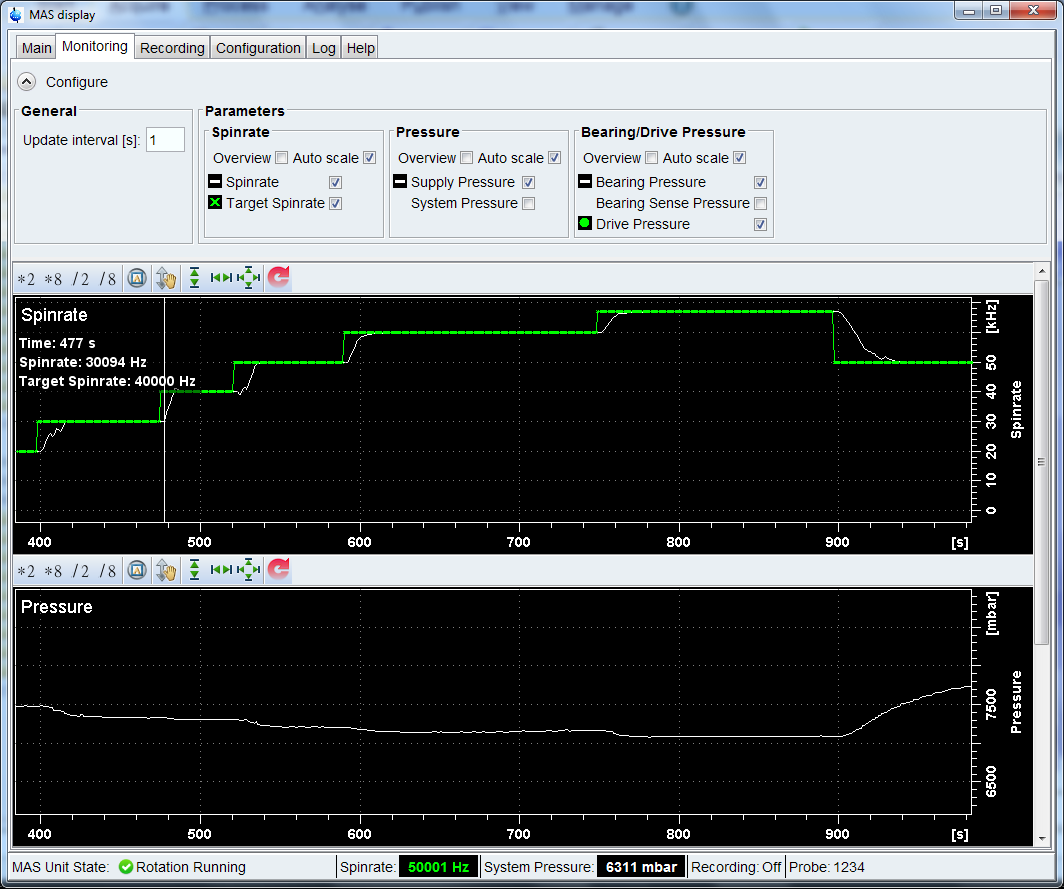
\includegraphics[width=8cm]{images/gruppe1_auf.png}
					\captionof{figure}{Erhöhen der Rotationsfrequenz}
					\label{fig:xray}
					\vspace*{4mm}
				\end{Figure}
				
				\loremlines{15}{4}
				
				\begin{Figure}
					\centering
					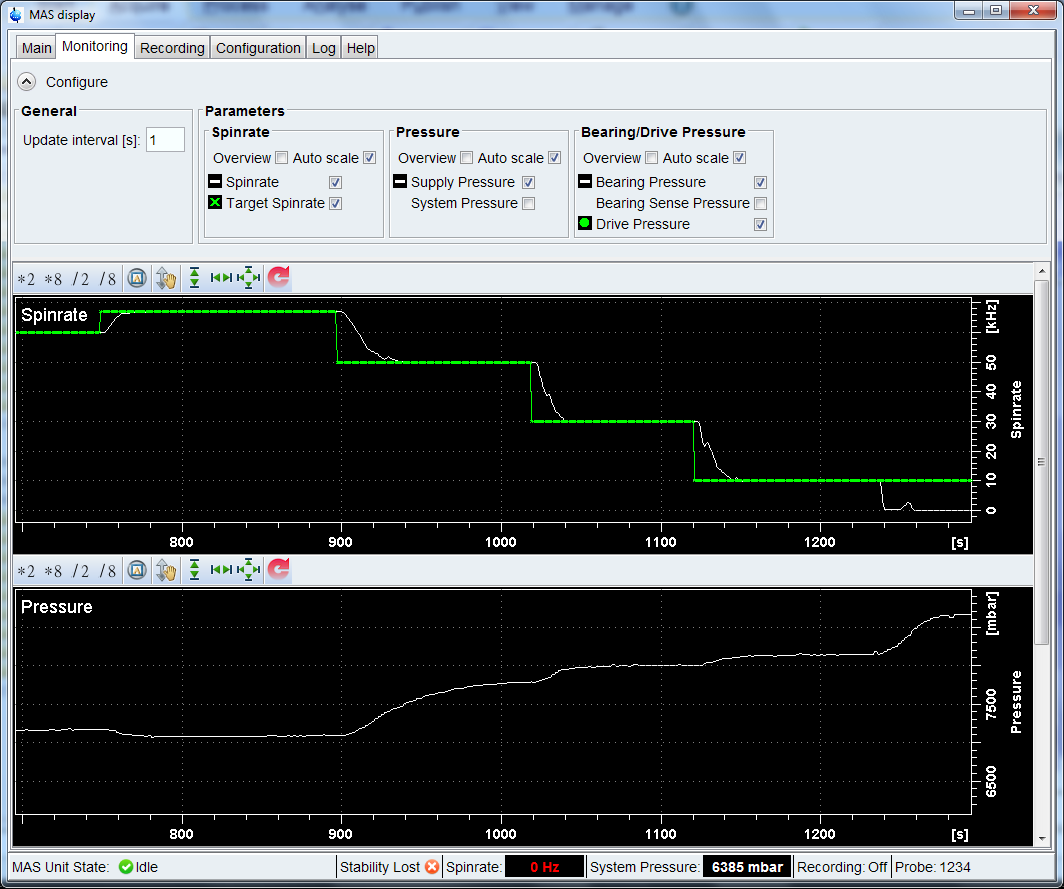
\includegraphics[width=8cm]{images/gruppe1_ab.png}
					\captionof{figure}{Erniedrigen der Rotationsfrequenz}
					\label{fig:xray}
					\vspace*{4mm}
				\end{Figure}
			
		\section{Spektrum in NMR-Software (Topspin) auswerten}
			\subsection{Resultate}
				\lipsum[66]
			
				\begin{Figure}
					\centering
					\begin{tikzpicture}
						\node[anchor=south west,inner sep=0] at (0cm,0cm) {
							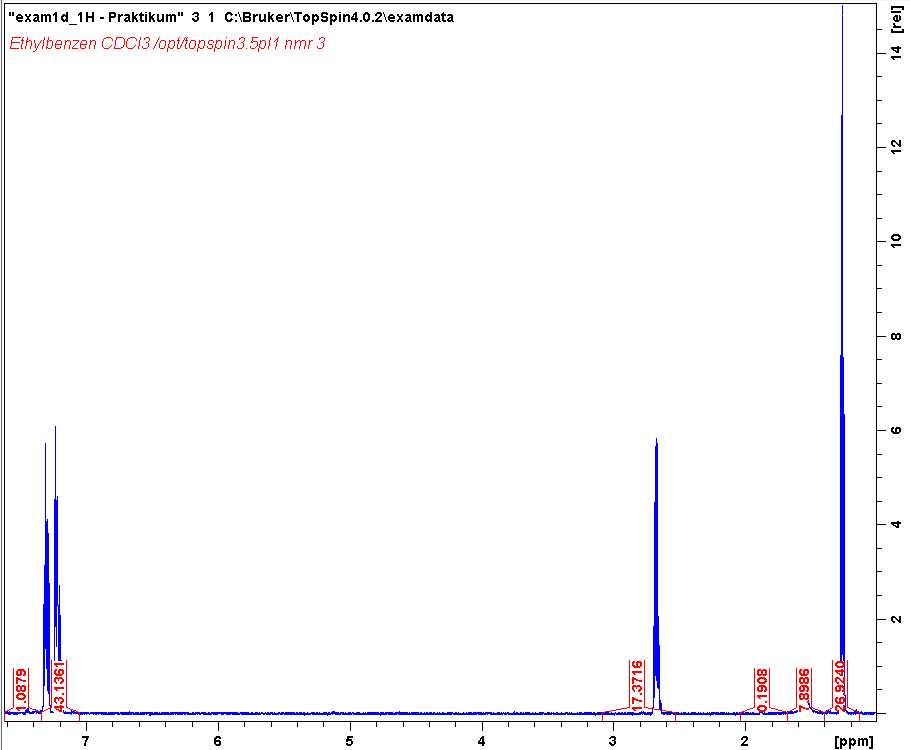
\includegraphics[width=7cm]{images/spektrum_crop.PNG}
						};
						\node (A1) at (0.4cm,3.5cm) {\huge I};
						\node[anchor=west] (A2) at (0.1cm,2.75cm) {\large Aromatischer Ring};
						\node (B1) at (5cm,3.5cm) {\huge II};
						\node (B2) at (5.1cm,2.75cm) {\large \chemfig{CH_2}};
						\node (C1) at (5.75cm,5.25cm) {\huge III};
						\node (C2) at (5.75cm,4.5cm) {\large \chemfig{CH_3}};
					\end{tikzpicture}
					\captionof{figure}{Gesamtspektrum von Ethylbenzen}
					\label{fig:ct}
					\vspace*{4mm}
				\end{Figure}
			
				\loremlines{1}{4}
			
				\begin{Figure}
					\centering
					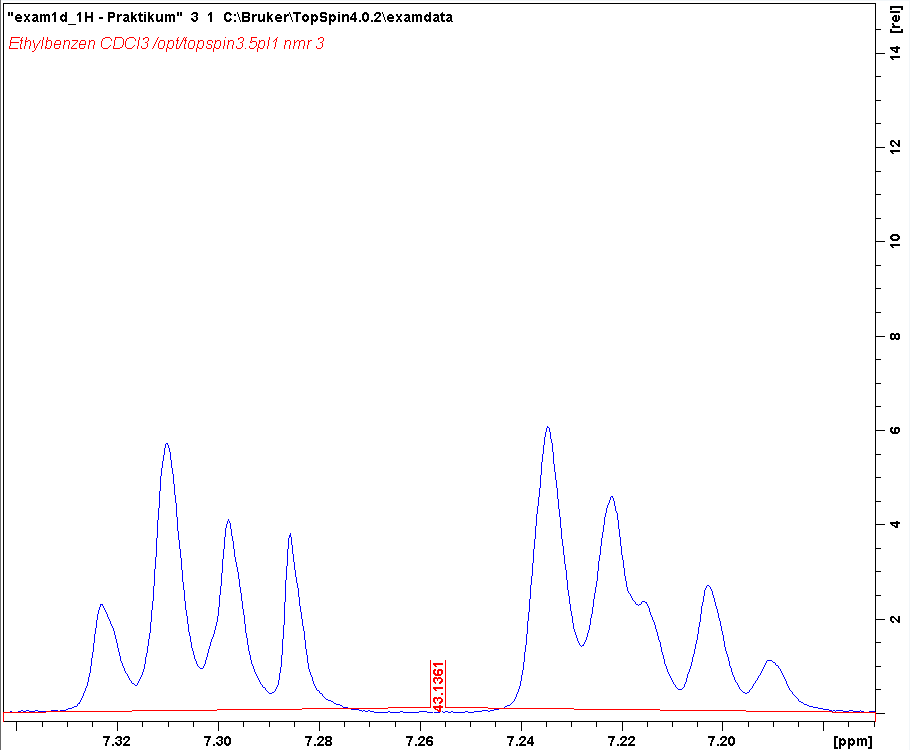
\includegraphics[width=7cm]{images/i_crop.PNG}
					\captionof{figure}{Spektrum vom Aromatischen Ring}
					\label{fig:ct}
					\vspace*{4mm}
				\end{Figure}
			
				\loremlines{2}{4}
				
				\begin{Figure}
					\centering
					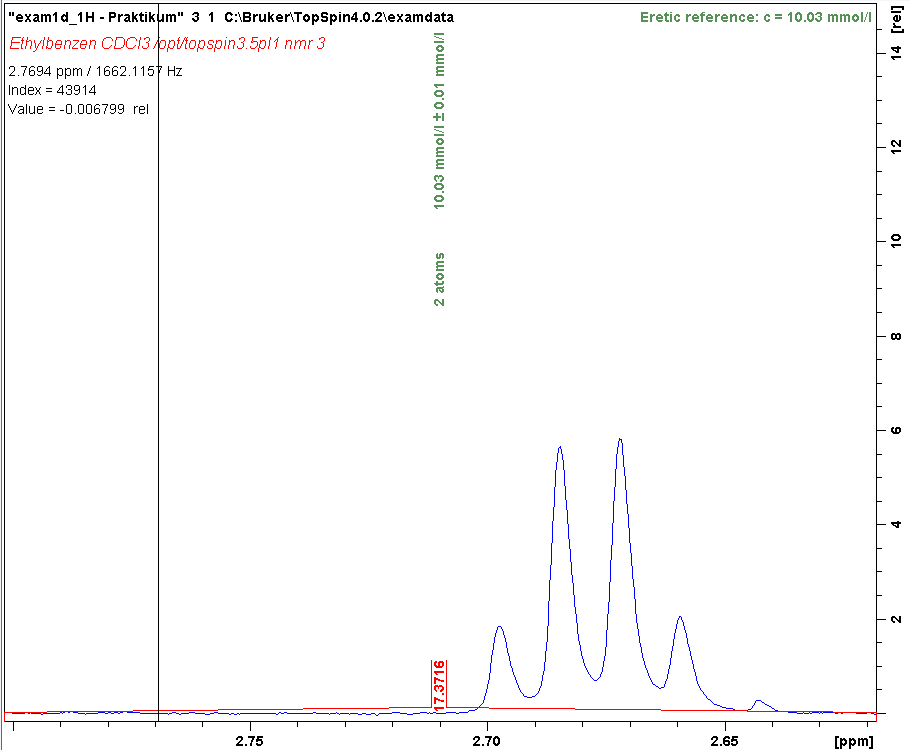
\includegraphics[width=7cm]{images/ii_crop.PNG}
					\captionof{figure}{Spektrum von $CH_3$}
					\label{fig:ct}
					\vspace*{4mm}
				\end{Figure}
			
				\loremlines{3}{4}
			
				\begin{Figure}
					\centering
					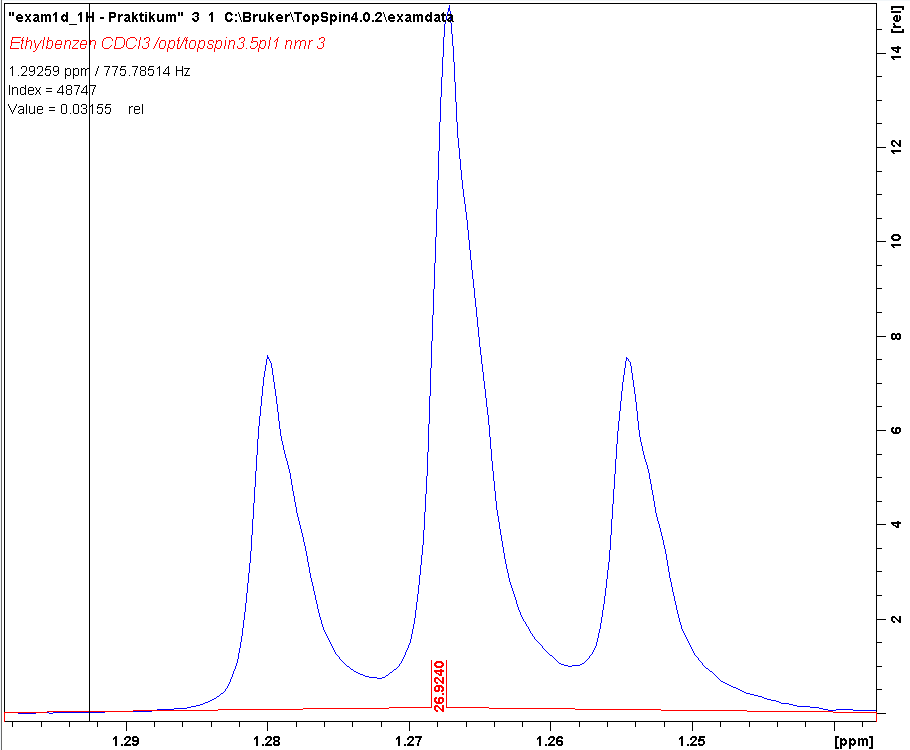
\includegraphics[width=7cm]{images/iii_crop.PNG}
					\captionof{figure}{Spektrum von $CH_2$}
					\label{fig:ct}
					\vspace*{4mm}
				\end{Figure}
				
				
	
			
	\end{multicols*}
\end{document}